\documentclass[toc]{../cs-classes/cs-classes}

\title{Operating Systems}
\author{Timothy Bourke\\ Notes by Antoine Groudiev}

\newcommand*{\option}{\texttt{ option}}
\newcommand*{\none}{\texttt{None}}
\newcommand*{\some}{\texttt{Some }}
\newcommand*{\vmap}{\texttt{VMAP}}

\begin{document}
\begin{abstract}    
    This document is Antoine Groudiev's class notes while following the class \emph{Systèmes d'exploitation} (Operating Systems) at the Computer Science Department of ENS Ulm. It is freely inspired by Timothy Bourke's classes, and especially its slides.
\end{abstract}

\section*{Introduction}
An operating system is made of three main parts: a \emph{kernel}, \emph{libraries}, and \emph{applications}. It is useful for sharing memory, computation time, processors, and devices (keyboards, disks, graphics cards, \dots). It constitues an abstraction layer used as a base for building bigger systems. For example, the OS allows hardware independence for applications, and provides common services (such as file systems with access control) and allows concurrency and communication with protection and access control.

The kernel contains lots of data structures and functions used for bookkeeping, as well as abstract modules such as interfaces, data structures, and functions for services. It allows a low-level control of hardware, and manages the concurrency and the events.

\section{Virtual Memory}
\subsection{Introduction}
We will start by studying the concept of \emph{virtual memory}. An OS must share finite ressources among multiple users and applications. It provides an abstraction for building such applications, which do not need to worry about the complexity of memory management with other applications. Indeed, physical memory must be shared: but what happens if it runs out, or if one process tries to read or write the memory of another? This is where virtual memory comes in handy: it allows to run each process in a virtual address space, and selectively share memory between processes for them to communicate. Furthermore, it allows processes to use faster physical memory as a cache for files on slower disks.

Virtual memory is an abstraction provided by a sophisticated and elegant mix of hardware and software. Hardware capabilities include exceptions (synchronous interrupts), address translation (which we will study in this section), main memory and caching of files on disks. Software-wise, we will study the kernel memory system. Hardware is needed to intervene at the lowest-level -- each individual \texttt{mov} instruction -- and for speed. Software is needed to implement sophisticated, flexible algorithms and for pervasive integration within a kernel.

For application programmers, virtual memory is largely invisible. Only very few programmers ever have to deal directly with this low-level hardware and software. Nevertheless, we will study it because it pervades all levels of a computer system; understanding how it works gives a deeper understanding of how the system works. It also provides powerful capabilities that can be exploited in applications. OS programmers cannot avoid knowing about virtual memory.

\subsection{Physical and virtual addressing}
Physical addressing is used in "simple" systems like embedded microcontrollers, in devices like cars, elevators, digital picture frames, \dots

Conversely, \emph{virtual addressing} is used in all modern servers, desktops, laptops and high-end mobile phones. It uses an MMU (Memory Management Unit), which translated the virtual address (VA) to a physical address (PA).

\subsection{Virtual memory address translation}
A \emph{virtual address space} is a set $V$ of $|V|=:N=2^n$ virtual addresses used within programs. These addresses are mapped to a \emph{physical address space}, which is a set $P$ of $|P|=:M=2^m$ physical addresses of DRAM.

The address translation can be formalised by a function $\vmap:V\to P \option$. For some virtual address $a$, we have
\begin{equation*}
    \vmap(a) = \begin{cases*}
        \some a' & if data at virtual address $a$ is at physical address a' in $P$\\
        \none & if data at virtual address $a$ is not in physical memory
    \end{cases*}
\end{equation*}
We can represent this simple model of the function \vmap by a data structure accessed by hardware (the MMU), and manipulated by software (the OS). 

We could think of individually mapping each byte or word, but it is too complicated in terms of software, and too expensive in terms of hardware and data structure. Thus, the address spaces are divided into numbered \emph{pages}, which are blocks of a specific size, e.g. 4 KiB. They are always aligned on \emph{page size}, i.e. they cannot overlap. The mapping is therefore represented by a \emph{page table}. In first approximation, it is a list of entries, one for each virtual page, specifing either \none (when there is no mapping), or $\some p$ where $p$ is a physical page number.

\subsection{VM as a tool for memory management}
The key idea is that each process has its own virtual address space. It can view memory as a simple linear array of bytes. Mapping function scatters addresses through physical memory. Well-chosen mappings simplify memory allocation and management. Each virtual page can be mapped to any physical page. A virtual page can be stored in different physical pages at different times. This allows to share code and data among processes, by mapping virtual pages to the same physical page.

\begin{figure}[!ht]
    \centering
    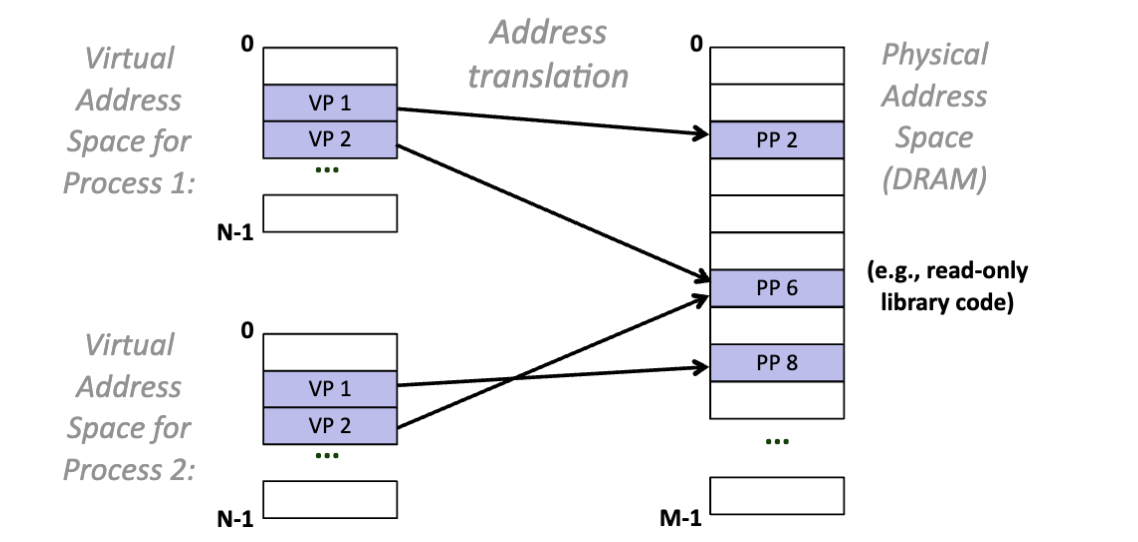
\includegraphics[scale=0.6]{images/address-translation.png}
    \caption{Address translation}
\end{figure}

\subsection{Address translation}
The following diagram shows the translation of addresses with a page table:
\begin{figure}[H]
    \centering
    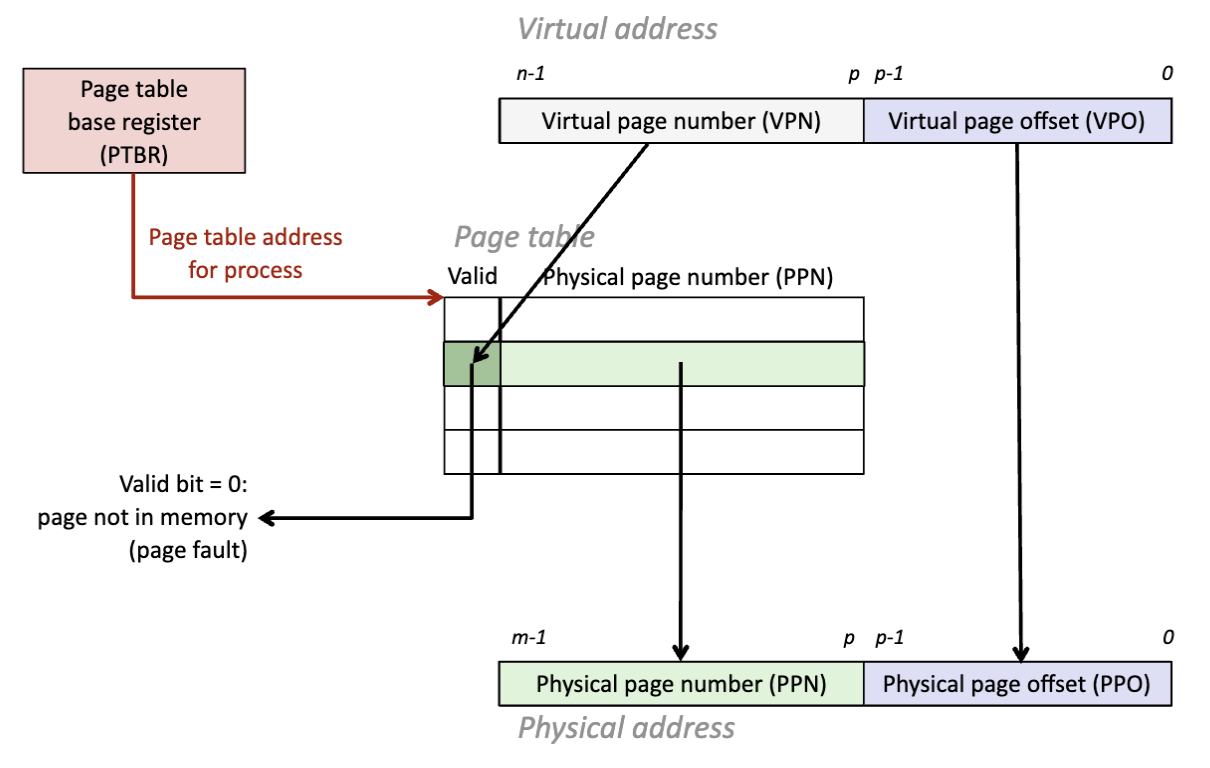
\includegraphics[scale=0.5]{images/virtual-addressing.png}
    \caption{Use of a page table}
\end{figure}

The processor stars by sending a virtual address to the MMU, which requests a page table entry address from memory. The page table entry is fetched from page table in memory, and the MMU sends the phydical address to cache or memory. Finally, the cache or memory sends the data word back to the processor. This is summarized in the following diagram:
\begin{figure}[H]
    \centering
    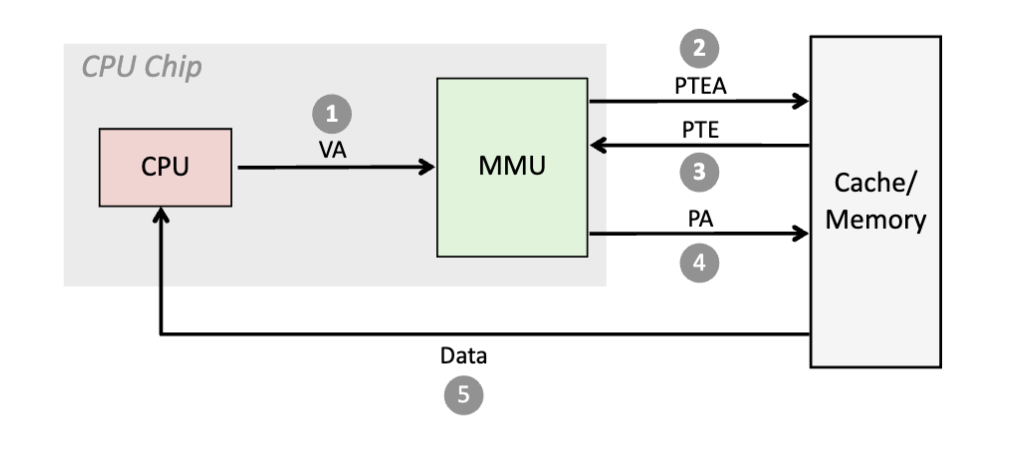
\includegraphics[scale=0.6]{images/MMU.png}
    \caption{Page hit}
\end{figure}

Translation can be sped up using a \emph{Translation Lookaside Buffer} (TLB). Page table entries (PTEs) are cached in L1 like any other memory word. PTE hit still requires a small L1 delay, and PTEs may be evicted by other data references. The solution to this is a \emph{Translation Lookaside Buffer} (TLB). It is a small hardware cache in the MMU, which maps virtual page numbers to physical page numbers. It contains complete page table entries for a small number of pages.
\begin{figure}[H]
    \centering
    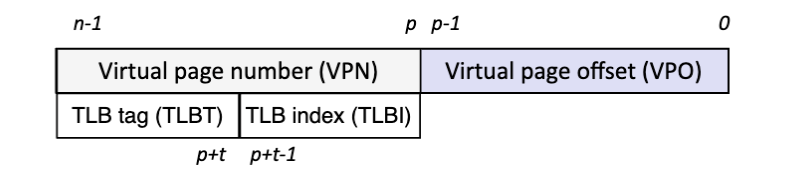
\includegraphics[scale=0.8]{images/TLB.png}
    \caption{Use of a Translation Lookaside Buffer (TLB)}
\end{figure}
The modified hit procedure using TLB is therefore of the form:
\begin{figure}[H]
    \centering
    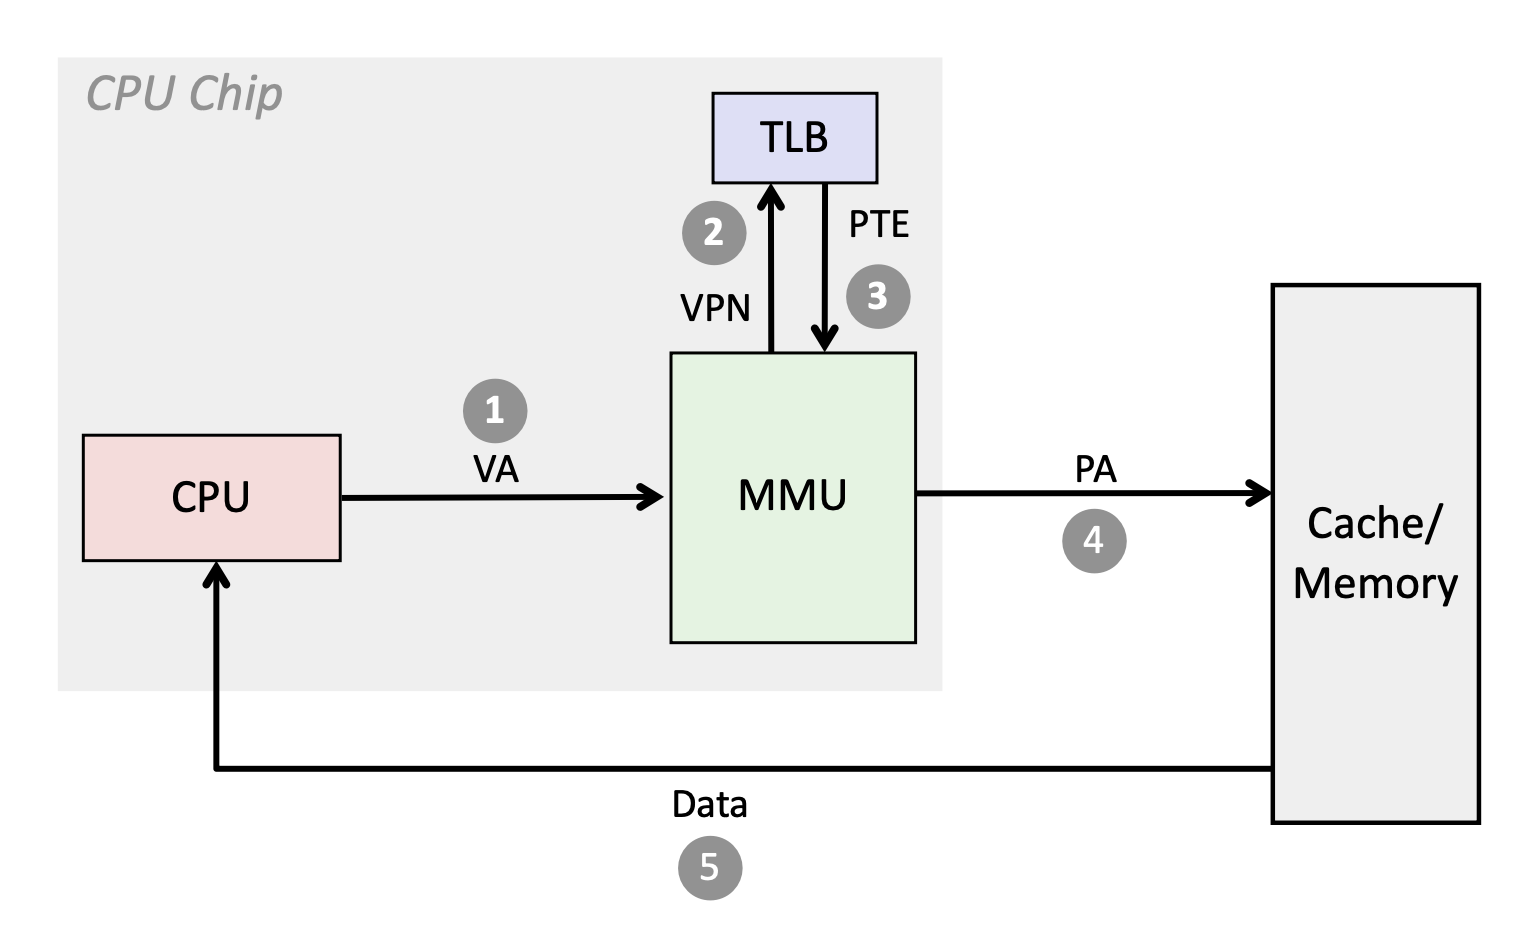
\includegraphics[scale=0.4]{images/TLB-hit.png}
    \caption{TLB hit}
\end{figure}
Notice that a TLB hit eliminates a memory access. A TLB miss incus an additional memory acces (the PTE). Fortunately, TLB misses are rare.
\begin{figure}[H]
    \centering
    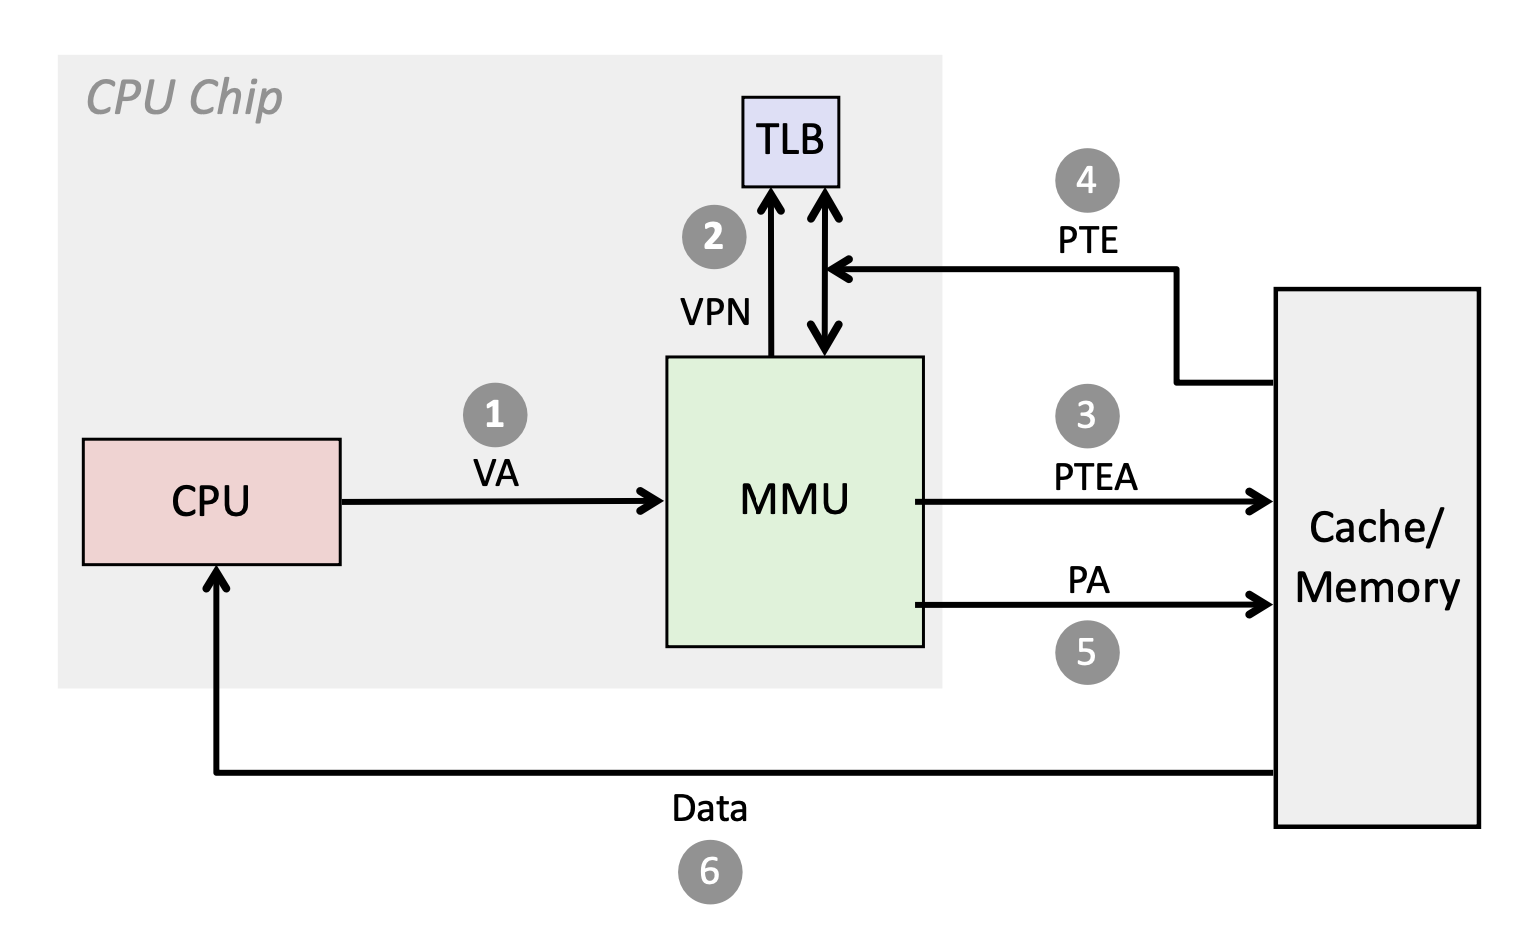
\includegraphics[scale=0.4]{images/TLB-miss.png}
    \caption{TLB miss}
\end{figure}

\subsection{Kernel and User Mode}
Each user process will have its own virtual address space define by a distinct page table. But should user code be allowed to update page tables and virtual memory mappings directly? No! That would not provide any real protection. Therefore, a process has at least 2 operating modes: a \emph{Kernel/Supervisor mode}, in which all instructions and registers are available, and a \emph{User mode}, in which some instructions and registers are restricted. Special instructions or events (interrupts) alloww to switch from one operating mode to the other. Virutal memory mappings can depend on the mode.

In practice, PTEs are extended with permission bits. Page permissions are checked for every move instruction to or from memory. If violated, the OS sends the process the error SIGSEGV (segmentation fault).
\begin{figure}[H]
    \centering
    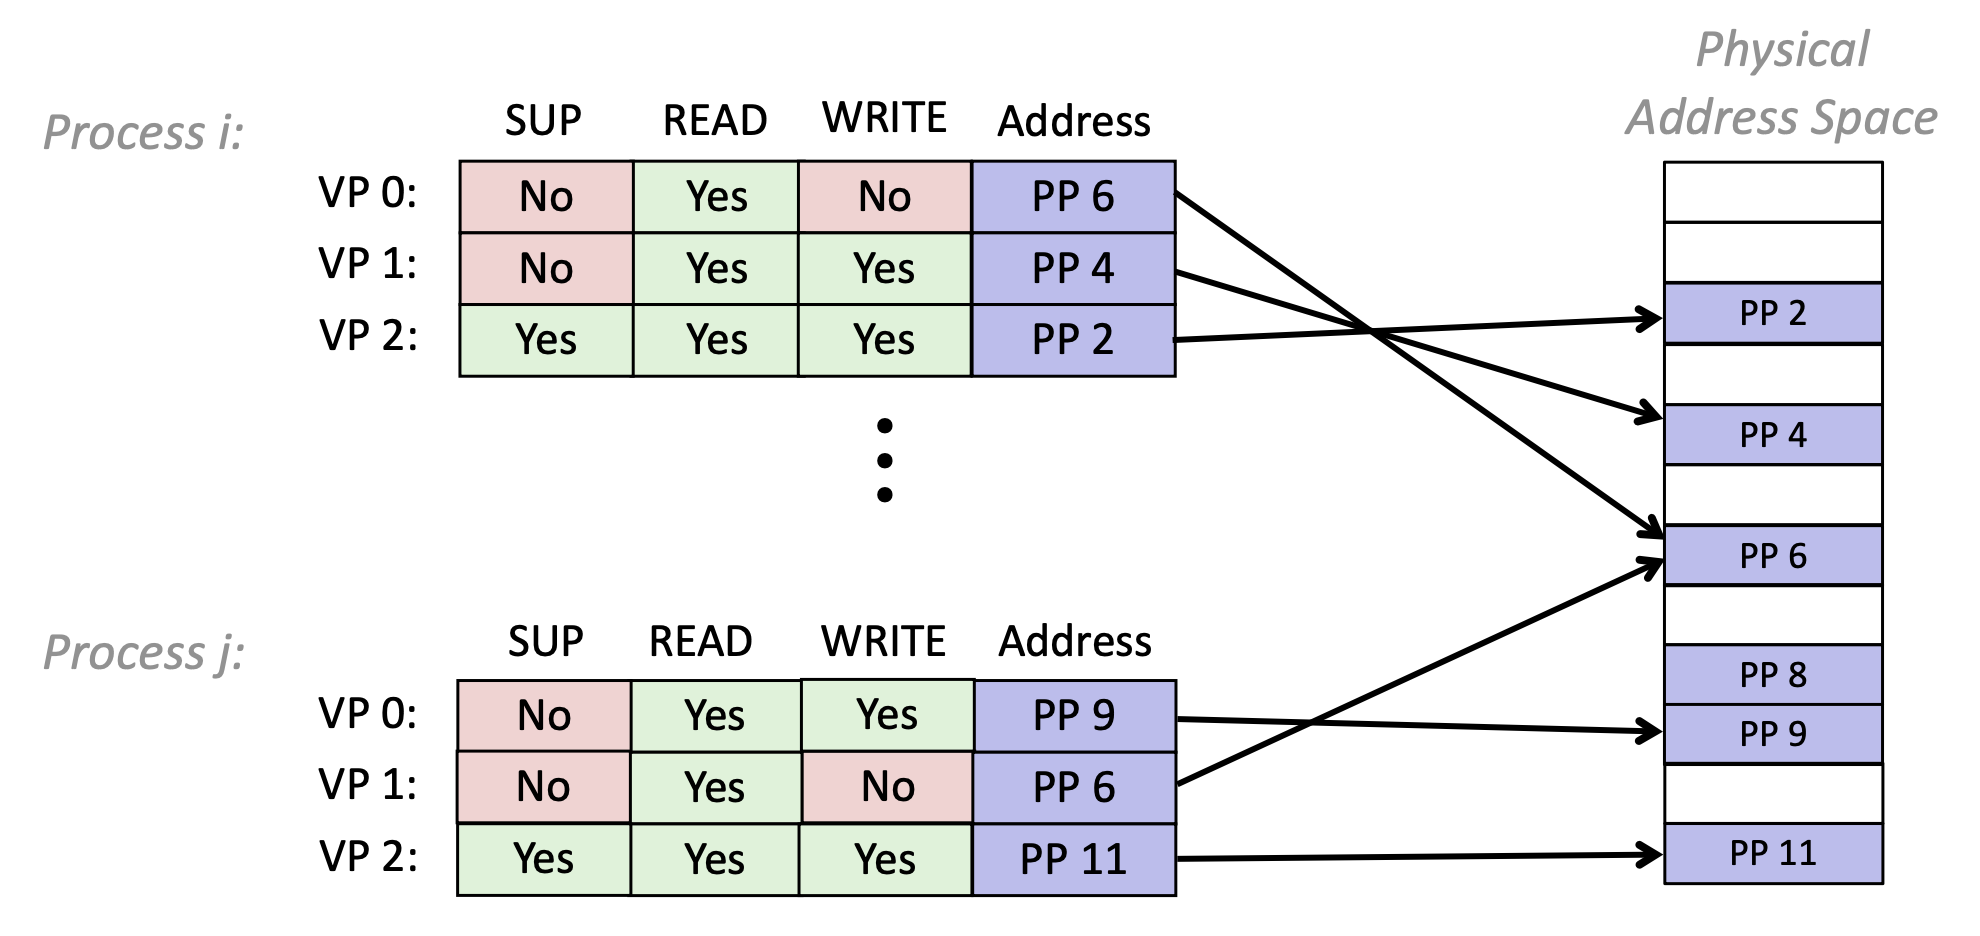
\includegraphics[scale=0.3]{images/PTEs-permissions.png}
    \caption{PTEs extended with permission bits}
\end{figure}

\subsection{Multi-level page tables}
Suppose that we maintain a 48-bit virtual address space, with a page size of 4 KiB ($2^{12}$), with an 8-byte PTE. We would need a 512 GiB page table:
\begin{equation*}
    2^{48} \times 2^{-12} \times 2^3 = 2^{39} \textnormal{ bytes}
\end{equation*}

\begin{figure}[H]
    \centering
    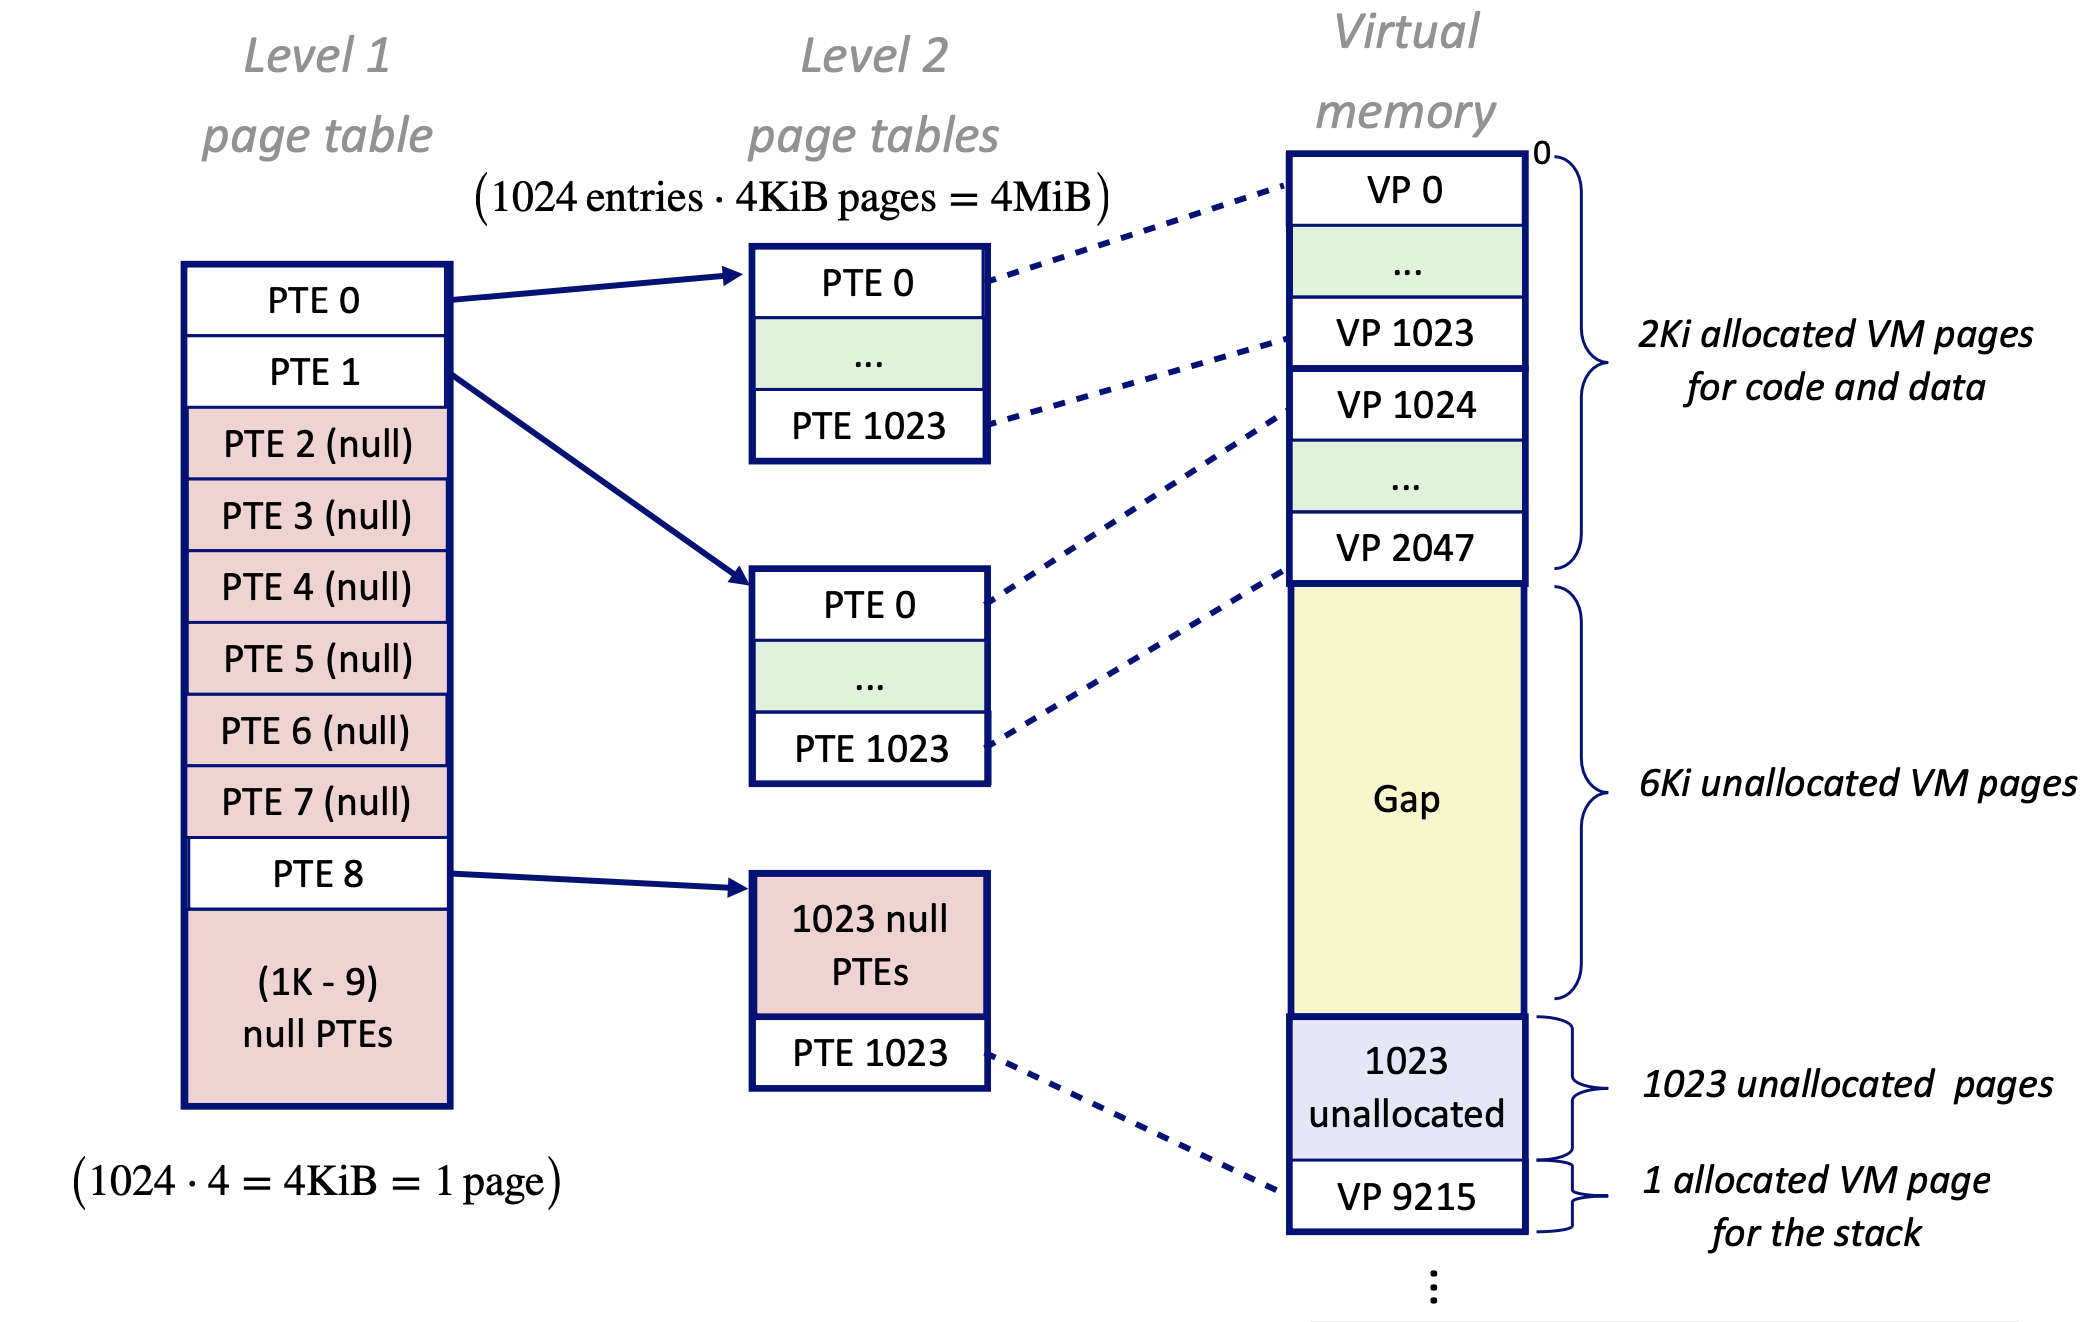
\includegraphics[scale=0.35]{images/2-level-PT.png}
    \caption{A two-level page table hierarchy}
\end{figure}
A solution to this is to use multi-level page tables. For example, we could use a 2-levels page table, where in the first level, each PTE points to a page table, and in the second level, each PTE points to a page. This reduces memory requirements. Usually, most of the virtual address space is unallocated. If a level 1 PTE is null, there is no corresponding level 2 page table. The level 2 page tables can be created as needed, reducing pressure on physical memory.

\begin{figure}[H]
    \centering
    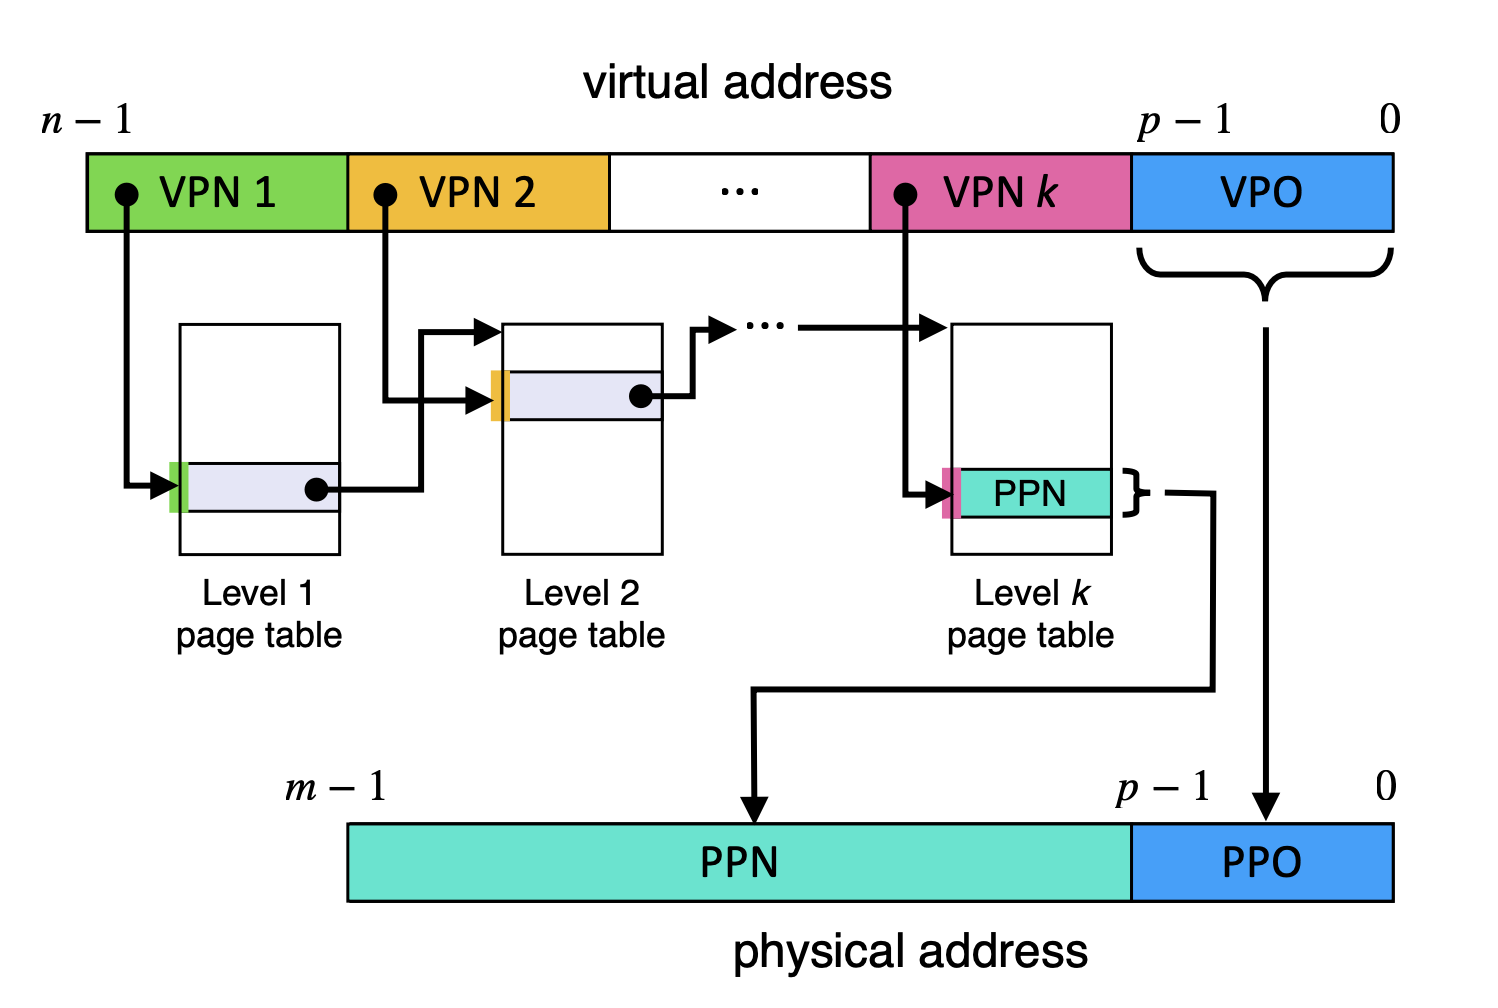
\includegraphics[scale=0.4]{images/translation-k-level.png}
    \caption{Address translation with a $k$-level page table}
\end{figure}
This may seem expensive and impractical, but the TLB helps by catching PTEs from the page tables at different levels, and in practice the lookup is not much slower than with a single level.

\subsection{x86 real mode and segment:offset addressing}
\subsubsection{Introduction}
The first Intel 16-bit processor, the 8086, was released in 1978. It uses 16-bit words and 20-bit addresses, allowing up to $2^{20}$=1 MiB of addressable memory. It uses memory segmentation, with no MMU: physical addressing is always used. The following 8088 and 80186 introduces some slight modifications and new instructions. They are the ancestors of the x86 architecture.

\subsubsection{The segment:offset addressing}
How can we access a 20-bit physical address space with 16-bit registers? It uses special segment registers to provide the extra 4 bits. For example, put 0x12F3 in the data segment register \texttt{\%ds}. This is the base address of the 64K segment starting at 0X12F30. Notice that the physical base address is the segment address shifted 4 bits to the left. Addresses in moste data instructions are implicitly relative to \texttt{\%ds}. For example, the instruction \texttt{movl 7, \%ax} loads the word from 0x12F37 into \texttt{\%ax}. Putting 0X4B27 in the \texttt{\%bx} register then executing \texttt{movl (\%bx), \%ax} loads the word from 0x12F30+0x4B27 into \texttt{\%ax}. Therefore, we have the equation:
\begin{equation*}
    \textnormal{physical address} = (\textnormal{segment address} << 4) + \textnormal{offset}
\end{equation*}

Different segment:offset addresses refer to the same physical address (e.g. both 0020:0010 and 0000:0210 refers to physical address 0x210). Furthermore, some addresses are too big for 20-bits (e.g. FFF:0010 wraps around to the beginning: 0X00000).

\subsubsection{Real mode}
All x86 and x86-64 start in real mode. They can only access 1 MiB, with no memory protection or virtual memory. They need segment registers to access more than 64K. Nevertheless, they can access BIOS functions to query and control hardware, and can still use 32-bit registers. The code that "boots" a kernel executes in real mode and later switches to protected mode by updating CPU registers. There exist techniques for running real-mode processes or switching back to real mode to access the BIOS.

The segment registers are the following:
\begin{figure}[H]
    \centering
    \begin{tabular}{|c|c|p{8cm}|}
        \hline
        \texttt{\%cs} & Code segment register & Used implicitly with the instruction pointer \texttt{\%ip}, and updated on calls, jumps, interrupts, and exceptions\\
        \hline
        \texttt{\%ds} & Data segment register & Used implicitly by most data access instructions\\
        \hline
        \texttt{\%es} & Extra segment register & Used implicitly in some string instructions\\
        \hline
        \texttt{\%fs} & Far segment register & Free for programmer use\\
        \hline
        \texttt{\%gs} & Far segment register & Free for programmer use\\
        \hline
        \texttt{\%ss} & Stack segment register & Used implicitly with the stack pointer \texttt{sp} and base pointer \texttt{bp}\\
        \hline
    \end{tabular}
    \caption{Segment registers}
\end{figure}
Apart from the implicit effects of the segment registers, programmers can also use them explicitly. For example, \texttt{movl \$4, \%fs=200} moves a 32-bit value representing the number 4 to the address given by the segment register \texttt{\%fs}, plus 200. Similaryl, \texttt(movl \$4, \%es:100(\%eax, \%ebx, 2)) moves a 32-bit value representing the number 4 to the address given by
\begin{equation*}
    \texttt{\%eax} + \texttt{\%ebx} \times 2 + 100
\end{equation*}
relative to the segment register \texttt{\%es}.

\subsubsection{Low-level real-mode programming}
The PC contains a set of firmware routines called the BIOS -- Basic Input/Output System. While many modern systems are based on the UEFI -- Unified Extensible Firmware Interface, most also support BIOS services.

The BIOS software executes when a computer is powered on. It checks the installed hardware and configures it. It provides features for configuring machine settings, and goes through the attached disks in order, loading their first sector into memory and checking for a special value. If the value is found, then the sector contents loaded into memory are execture in real mode. This small (512 bytes) program is normally responsible for loading and executing the next boot stage and ultimately the kernel software.

The firmware contains routines that can be called from real mode by setting certain registers and triggering an interrupt, e.g.
\begin{minted}{asm}
    mov $0x0e, %ah
    mov '!', %al
    int $0x10
\end{minted}
specifies the teletype function (0x0e) with argument '!', and triggers the "video service" interrupt to display the character. It is time-consuming to experiment with such low-level programs on real hardware, but it is realtively easy to do in an emulator such as \texttt{qemu} or \texttt{Bochs}.

\subsection{x86 protected mode and memory segmentation}

\subsection{x86-64 long mode}

\subsection{x86 and x86-64 paging}

\end{document}